\documentclass[20pt,landscape]{foils}
\usepackage{amsmath, amssymb, amsthm}
\usepackage{color}
\usepackage{hyperref}
%\usepackage{pause}
\usepackage{graphicx}
\usepackage{epsfig}
%\usepackage{geometry}
%\geometry{headsep=3ex,hscale=0.9}
\newcommand{\bd}{\textbf}
\newcommand{\no}{\noindent}
\newcommand{\un}{\underline}
\newcommand{\bi}{\begin{itemize}}
\newcommand{\ei}{\end{itemize}}
\newcommand{\be}{\begin{enumerate}}
\newcommand{\ee}{\end{enumerate}}
\newcommand{\bc}{\begin{center}}
\newcommand{\ec}{\end{center}}
\newcommand \h {\hspace*{.3in}}
\newcommand{\bul}{\hspace*{.3in}{\textcolor{red}{$\bullet$ \ }}}
\newcommand{\xbar}{\bar{x}}
\rightheader{Stat 330 (Fall 2016): slide set 6}

\begin{document}
\LogoOff

\foilhead[1.3in]{}
\centerline{\LARGE \textcolor{blue}{Slide set 6}}
\vspace{0.3in}
\centerline{\large Stat 330 (Fall 2016)}
\vspace{0.2in}
\centerline{\tiny Last update: \today}
\setcounter{page}{0}

\foilhead[-.8in]{\textcolor{blue}{Total Probability Law and Bayes' Rule}}
\no {\textcolor{magenta}{Experiment: }}{\textcolor{cyan}{Treasure Hunt}}\\[.1in]
\no \bul {\textcolor{cyan}{Box 1  has two gold coins}}\\[.1in]
\no \bul {\textcolor{cyan}{Box 2  has one gold coin and one silver. }}\\[.1in]
\no \bul {\textcolor{cyan}{Box 3  has two silver coins.}}\\[.1in]
\no \bul {\textcolor{cyan}{Suppose that you select one of the boxes randomly and then select one of the 
coins from this box. What is the probability that the coin you select is a gold coin?}}\\[.2in]
\no For a problem like this, that consists of a step-wise procedure, it is 
often useful to draw a tree (a flow chart) of the choices we can make 
in each step.\\[.15in]
\no Define $B_1, B_2, B_3$ to be the events that Box 1, 2 or 3 is selected randomly.

\foilhead[-.8in]{\textcolor{blue}{Treasure Hunt... continued}}
\no  {\textcolor{cyan}{A tree diagram shows all possible outcomes of this two-step procedure:}}\\[.01in]  
\centerline{\includegraphics*[scale=0.45]{box_coin_tree.pdf}}\\[.01in]
\no Choosing one box (at random) means, that all boxes are equally likely 
to be chosen: $P(B_{i}) = \frac{1}{3}$ for $i = 1,2,3$.\\[.1in]
\no $P(\text{Select a gold coin}| B_1) = 1$. Why?\\[.1in]
\no $P(\text{Select a gold coin}| B_2) = 0.5$. Why?\\[.1in]
\no Define new events  $E_1$ and $E_2$:\\[.1in]
\no $E_{1}= $ \text{ choose Box 1 and pick  a gold coin} \\[.1in]
\no $E_{2}= $ \text{ choose Box 2 and pick a gold coin} 
\foilhead[-.75in]{\textcolor{blue}{Treasure Hunt... continued}}
\no We use the definition of {\textcolor{magenta}{conditional probability}} to get $P(E_1)$ and $P(E_2)$!\\[.15in]
%
\no $ P(E_{1}) = P( \text{ choose Box 1 and pick a gold coin} )$\\[.1in]
 \hspace*{1in}$ = P(\text{ pick a gold coin } | B_{1}) \cdot  P(B_1) =  1 \cdot \frac{1}{3} =\frac{1}{3}.$ \\[.25in]
\no $P(E_{2}) = P( \text{ choose Box 2 and pick a gold coin } )$\\[.1in]
 \hspace*{1in} $=  P(\text{ pick a  gold coin } | B_{2})\cdot P(B_2) =  \frac{1}{2} \cdot \frac{1}{3} 
  = \frac{1}{6}. $\\[.2in]
\no The probability to choose a gold coin is the sum of $P(E_{1})$ and 
$P(E_{2})$ \\[.1in]
\no  {\textcolor{magenta}{This is because those are the only ways to get a gold coin, as we've seen in the tree diagram and they are mutually exclusive (disjoint)!}} \\[.1in]
Thus we have:\\[.1in]
 \hspace*{1.5in} $P( \text{ gold coin }) = \frac{1}{3} + \frac{1}{6} = 0.5.$\\[.1in]
\no We just used the {\textcolor{magenta}{Law of Total Probability}} to compute
the probability of choosing a gold coin.

\foilhead[-.75in]{\textcolor{blue}{Law of Total Probability}}
\no {\textcolor{magenta}{Definition.}} A collection of events $B_{1}, \ldots B_{k}$ is called a {\textcolor{magenta}{\emph{cover}}} or {\textcolor{magenta}{\emph{partition}}} of $\Omega$ if \\[.1in]
\no \textbf{(i)} the events are mutually exclusive (i.e., $B_{i}\cap B_{j} = \emptyset$ for $i\neq j$), and \\[.1in]
\no \textbf{(ii)} the union of the events is $\Omega$ (i.e., $\bigcup_{i=1}^{k}B_{i} = \Omega$). \\[.2in]
\no \bul We can represent a cover using a Venn diagram:\\[.1in]
    \centerline{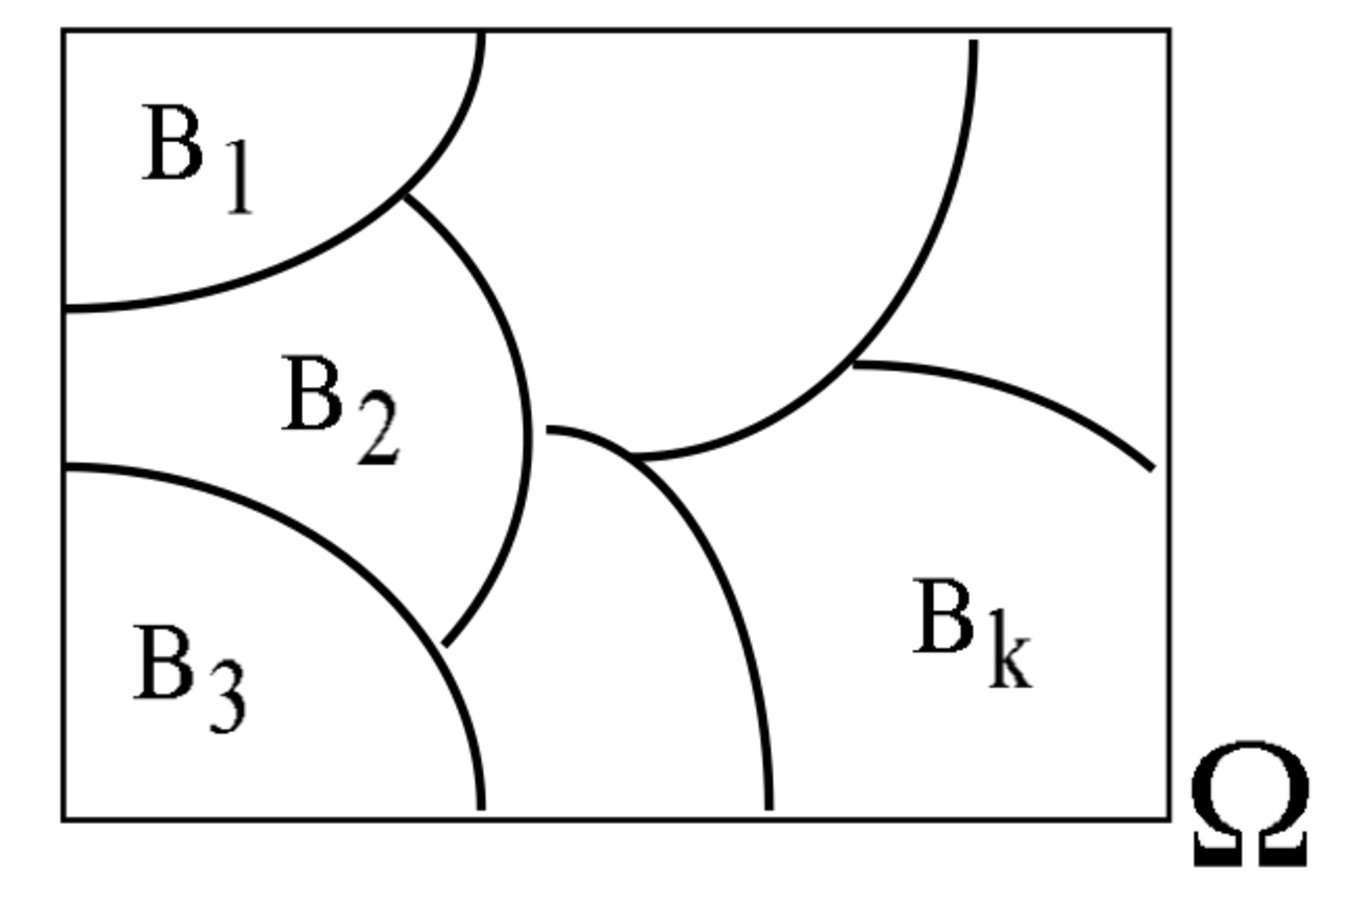
\includegraphics[width=2.5in]{cover.pdf}} \\[.01in]
\no \bul If we represent a multi-step procedure with a tree diagram, then the branches of the tree form a cover.

\foilhead[-.75in]{\textcolor{blue}{Law of Total Probability (continued...)}}
\no {\textcolor{magenta} {Theorem: \emph{Law of Total Probability.}}} If  the collection of events $B_{1}, \ldots, B_{k}$ is a cover of $\Omega$, and $A$ is an event, then 
$$P(A) = \sum_{i=1}^{k}P(A|B_{i})P(B_{i}).$$
\no {\textcolor{magenta} {Proof of the Law of Total Probability:}}\\[-.5in]
\begin{itemize}
\addtolength{\itemsep}{-0.6\baselineskip}
\item[\bul] By definition of conditional probability $P(A|B_{i})P(B_{i}) = P(A\cap B_{i})$
\item[\bul] Because $B_{1}, \ldots, B_{k}$ partition $\Omega$, the events $A\cap B_{1}, \ldots A\cap B_{k}$ are disjoint, and $\cup_{i=1}^{k}A_{i} = A$ where $A_i= A\cap B_i$. 
\item[\bul] By Axiom (iii) (slide set 2 p.5), $P(A) = \sum_{i=1}^{k}P(A\cap B_{i}) = \sum_{i=1}^{k}P(A|B_{i})P(B_{i})$. 
\end{itemize}
\foilhead[-.8in]{\textcolor{blue}{Law of Total Probability (continued...)}}
\no  We can depict event $A$ using a Venn diagram:\\[.1in]
    \centerline{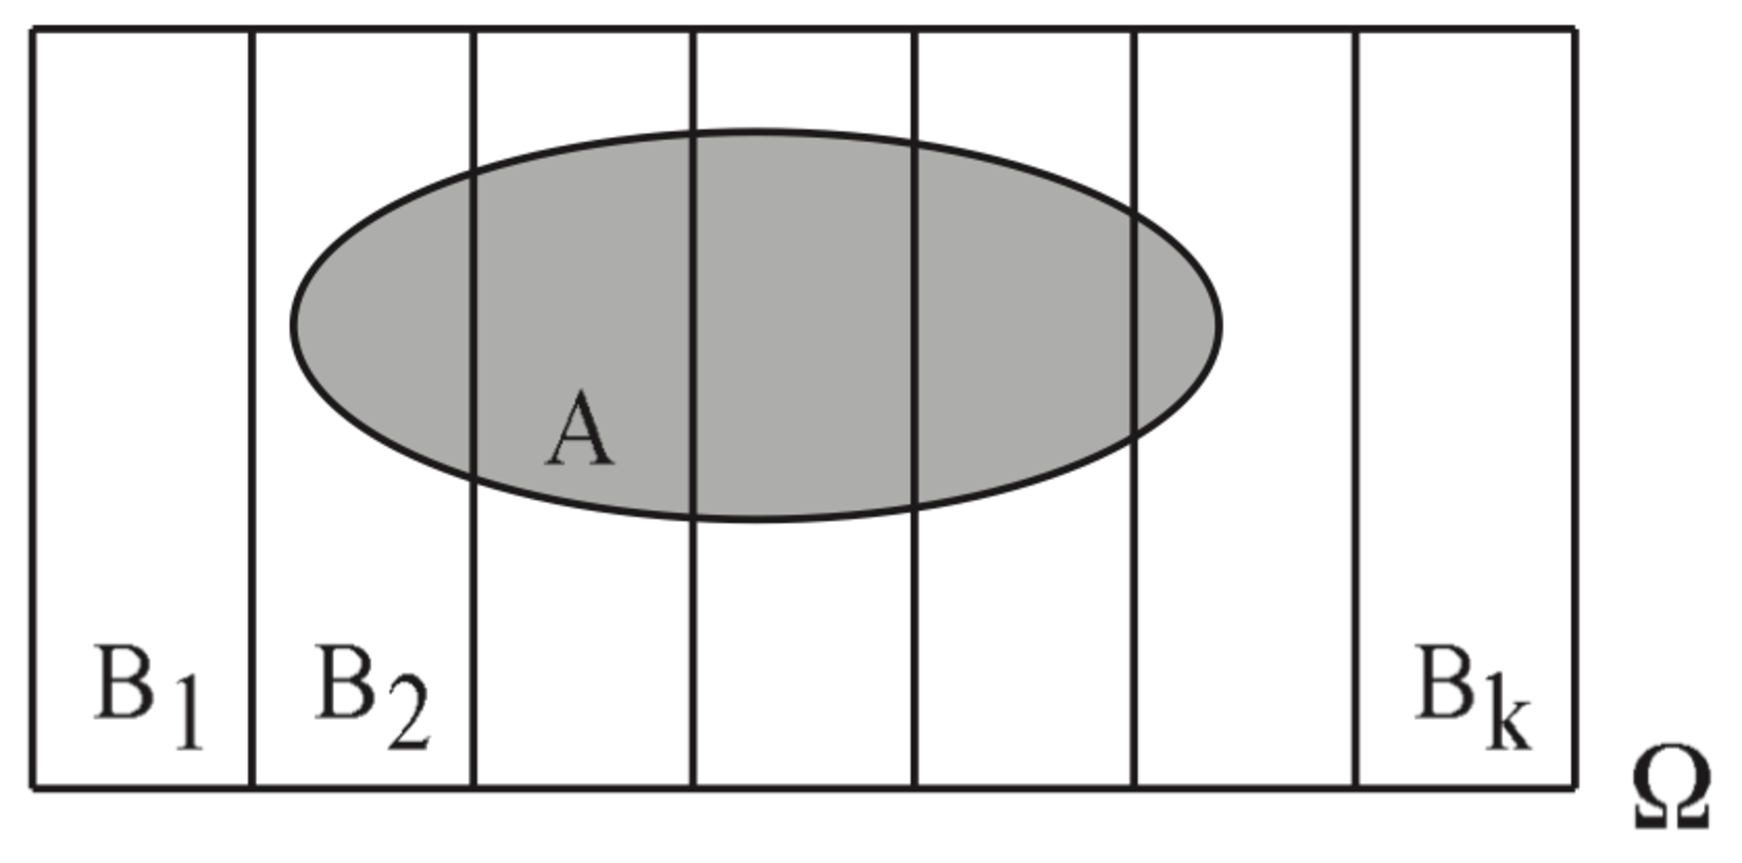
\includegraphics[width=3in]{total-prob.pdf}} \\[.01in]
\no The probability of event $A$ is put together as sum of the probabilities of the intersections $\sum_{i=1}^{k}P(A\cap B_{i})$.\\[.1in]
\no In our Treasure Hunt example, the events $B_1, B_2,$ and $B_3$ form a cover $\Omega$, as a coin can be drawn only from one of the boxes.\\[.1in]
\no Defining event $A=$ drawing a gold coin, we have\\[.15in]
 $P(A) = P(A|B_1)P(B_1)+P(A|B_2)P(B_2)= 1   \cdot \frac{1}{3}+ \frac{1}{2}  \cdot  \frac{1}{3}=0.5$ as before.\\[.15in] 
\no Note that event $A$ does not intersect the event $B_3$ as there are no gold coins in Box 3.



\foilhead[-.75in]{\textcolor{blue}{Bayes' rule.  }}
\no {\textcolor{magenta} {Theorem: \emph{Bayes' Rule.}}} If $B_{1}, \ldots, B_{k}$ is a cover or partition of $\Omega$, and $A$ is an event, then 
$$
P(B_{j}|A) = \frac{P(A|B_{j})P(B_{j})}{\sum_{j=1}^{k}P(A|B_{j})P(B_{j})}.
$$
\no {\textcolor{magenta} {Proof of Bayes' Rule:}}\\[-.5in]
\begin{eqnarray*}
P(B_{j}|A) &=& \frac{P(B_{j}\cap A)}{P(A)}= \frac{P(A|B_{j})P(B_{j})}{P(A)}\\ 
&=& \frac{P(A|B_{j})P(B_{j})}{\sum_{j=1}^{k}P(A|B_{j})P(B_{j})}.
\end{eqnarray*}
%\no We can represent Bayes' rule with tree diagrams and Venn diagrams as well. \\[.15in]
%\no {\textcolor{magenta}{Read Section 1.7 (Hofmann notes)}}.
\foilhead[-.8in]{\textcolor{blue}{ Example 1.7.3: (Hofmann notes) }}
\no {\textcolor{cyan} {A given lot of chips contains 2\%  defective chips. Each chip is tested before delivery.
However, the tester is not wholly reliable:
\begin{eqnarray*}
    P(\text{ ``tester says chip is good'' } | \text{  ``chip is good'' }) &=& 0.95 \\
    P(\text{ ``tester says chip is defective'' } | \text{ ``chip is defective'' }) &=&  0.94     
\end{eqnarray*}
If the test device says the chip is defective, what is the probability that the chip actually is defective?}}

\no We will apply Bayes' Rule, using  $C_{d}$, and $\bar{C}_{d}$ as cover.
\begin{eqnarray*}
    P(\underbrace{\text{ chip is defective }}_{:= C_{d}} &|& 
    \underbrace{\text{ tester says it's defective }}_{:= T_{d}})\\
    & =& P(C_{d}| T_{d}) 
 \end{eqnarray*}   
\foilhead[-.8in]{\textcolor{blue}{Continue Example 1.7.3 }}  
 \begin{eqnarray*}
P(C_{d}| T_{d})  
 &=&\frac{P(T_d|C_d)P(C_d)}{P(T_d)}\\
    &=& \frac{P(T_{d}| C_{d}) P(C_{d})}{P(T_{d}| C_{d}) P(C_{d}) + 
    P(T_{d}| \bar{C_{d}}) P(\bar{C_{d}})}\\
    &=&\frac{0.94\cdot 0.02}{0.94\cdot 0.02+(1-P(\bar{T}_d|\bar{C}_d))\cdot 0.98}\\
  &=  &\frac{0.94\cdot 0.02}{0.94\cdot 0.02+(1-0.95)\cdot 0.98}=0.28
\end{eqnarray*}

%eqnarray\no {\textcolor{magenta}{Study Example 2.3.2 of Baron's text carefully.}}


\end{document}
\end{document}





